% SC3270 --- Chapter 2: Preconditions and Postconditions: Writing Contracts (0->100 ground-up)
\chapter{Preconditions and Postconditions: Writing Contracts}
\label{ch:prepost}

\begin{quote}
\emph{``A function is a contract: if you give me this, I promise that.''} Preconditions are what the caller must achieve; postconditions are what the callee guarantees in return.
\end{quote}

\noindent\fbox{\parbox{\dimexpr\linewidth-2\fboxsep-2\fboxrule}{%
\textbf{From zero: no contract experience assumed.} We build contracts from English to logic, show why strong and weak matter, and prove that precondition-strengthening and postcondition-weakening are safe. Every notion is illustrated on tiny programs before formal rules.}}
\vspace{0.4em}

\section*{Learning Outcomes}
After this chapter you will be able to:
\begin{enumerate}[label=(L\arabic*)]
    \item formalise informal requirements as pre/post assertions with quantifiers;
    \item compare contract strength and order them by implication;
    \item apply precondition strengthening and postcondition weakening soundly;
    \item detect vacuous, too-weak, and too-strong specifications;
    \item write JML-style \texttt{requires/ensures} and class invariants.
\end{enumerate}

% ============================================================
\section{Contracts Before Code}
\label{sec:contracts}
\paragraph{Intuition.} A vending machine says ``insert 1.20\,€, press B3, receive cola.'' The \emph{requires} is ``you inserted 1.20\,€ and B3 is in stock''; the \emph{ensures} is ``you receive cola and change is correct.'' If you violate requires (insert 0.50\,€), the machine may do anything—keep money, return error—no guarantee.

A program function is identical:
\begin{center}
\texttt{requires $P$}\quad\texttt{function $f(x)$}\quad\texttt{ensures $Q$}
\end{center}
The caller must make $P$ true before the call; the function must make $Q$ true after, provided it terminates. The Hoare triple $\{P\}\,f\,\{Q\}$ is exactly this contract.

\begin{figure}[h]\centering
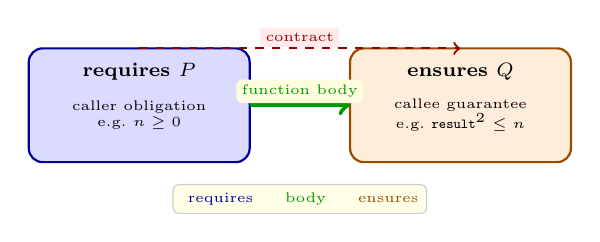
\begin{tikzpicture}[scale=0.85,font=\scriptsize]
\draw[fill=blue!14,draw=blue!60!black,thick,rounded corners=5pt] (0,0) rectangle (3.3,1.7);
\node at (1.65,1.35) {\textbf{requires $P$}};
\node[font=\tiny,align=center] at (1.65,0.70) {caller obligation\\e.g.\ $n\ge0$};
\draw[fill=orange!14,draw=orange!60!black,thick,rounded corners=5pt] (4.8,0) rectangle (8.1,1.7);
\node at (6.45,1.35) {\textbf{ensures $Q$}};
\node[font=\tiny,align=center] at (6.45,0.70) {callee guarantee\\e.g.\ $\texttt{result}^2\le n$};
\draw[->,ultra thick,green!60!black] (3.3,0.85) -- (4.8,0.85) node[midway,above,font=\tiny,fill=yellow!12,rounded corners=2pt,inner sep=2pt] {function body};
\draw[->,thick,red!60!black,dashed] (1.65,1.70) -- (6.45,1.70) node[midway,above,font=\tiny,fill=red!08,inner sep=2pt] {contract};
\node[font=\tiny,align=left,fill=yellow!10,draw=gray!40,rounded corners=2pt,inner sep=3pt] at (4.05,-0.55) {\textcolor{blue!60!black}{$\blacksquare$ requires} \quad \textcolor{green!60!black}{$\blacksquare$ body} \quad \textcolor{orange!60!black}{$\blacksquare$ ensures}};
\end{tikzpicture}
\caption{A contract as a bridge: the caller builds $P$, the body carries across, the caller may assume $Q$. Violate $P$ and the bridge has no deck.}
\label{fig:contract-bridge}
\end{figure}

\begin{definition}[Contract]
A \emph{contract} for command $C$ is a pair $(P,Q)$ of assertions. $C$ \emph{satisfies} it iff $\{P\}\,C\,\{Q\}$ holds. $P$ is the \emph{precondition}, $Q$ the \emph{postcondition}. When $C$ is a function with parameters $\bar{x}$ and result $r$, we write free variables accordingly.
\end{definition}

\begin{example}[Square root spec]
Informal: ``$\texttt{isqrt}(n)$ returns the integer square root of $n$.'' Formal:
\[
\{n\ge0\}\;\; r:=\texttt{isqrt}(n)\;\; \{r\ge0\ \land\ r^2\le n\ <\ (r+1)^2\}.
\]
Without $n\ge0$, no integer $r$ satisfies the post when $n=-1$—the spec would be unsatisfiable and any implementation vacuously ``correct'' on negative inputs, hiding the bug that caller and callee disagree on domain.
\end{example}

% ============================================================
\section{Strength: Weaker and Stronger}
\label{sec:strength}
Assertions ordered by $\Rightarrow$ form a lattice. Recall: $P$ is \emph{stronger} than $P'$ if $P\Rightarrow P'$ (fewer states satisfy it). $P$ is \emph{weaker} if $P'\Rightarrow P$. Strong $=$ small set, weak $=$ large set.

\begin{figure}[h]\centering
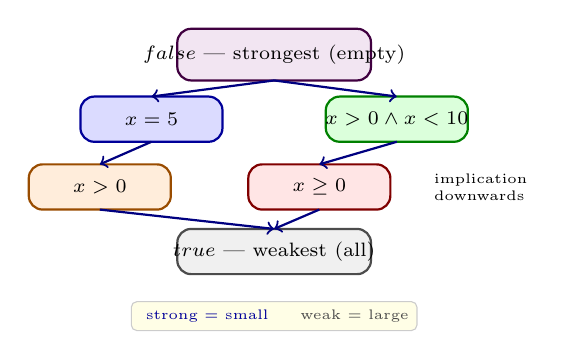
\begin{tikzpicture}[scale=0.82,font=\scriptsize]
\draw[fill=violet!10,draw=violet!50!black,thick,rounded corners=5pt] (2.5,3.0) rectangle (5.5,3.8);
\node at (4.0,3.40) {$\text{false}$ --- strongest (empty)};
\draw[fill=blue!14,draw=blue!60!black,thick,rounded corners=5pt] (1.0,2.05) rectangle (3.2,2.75);
\node at (2.1,2.40) {$x=5$};
\draw[fill=green!14,draw=green!50!black,thick,rounded corners=5pt] (4.8,2.05) rectangle (7.0,2.75);
\node at (5.9,2.40) {$x>0\land x<10$};
\draw[fill=orange!14,draw=orange!60!black,thick,rounded corners=5pt] (0.2,1.00) rectangle (2.4,1.70);
\node at (1.30,1.35) {$x>0$};
\draw[fill=red!10,draw=red!50!black,thick,rounded corners=5pt] (3.6,1.00) rectangle (5.8,1.70);
\node at (4.70,1.35) {$x\ge0$};
\draw[fill=gray!12,draw=gray!60!black,thick,rounded corners=5pt] (2.5,0.00) rectangle (5.5,0.70);
\node at (4.0,0.35) {$\text{true}$ --- weakest (all)};
\draw[->,thick,blue!50!black] (4.0,3.00) -- (2.1,2.75);
\draw[->,thick,blue!50!black] (4.0,3.00) -- (5.9,2.75);
\draw[->,thick,blue!50!black] (2.1,2.05) -- (1.30,1.70);
\draw[->,thick,blue!50!black] (5.9,2.05) -- (4.70,1.70);
\draw[->,thick,blue!50!black] (1.30,1.00) -- (4.0,0.70);
\draw[->,thick,blue!50!black] (4.70,1.00) -- (4.0,0.70);
\node[font=\tiny,align=left] at (7.2,1.35) {implication\\ downwards};
\node[font=\tiny,align=left,fill=yellow!10,draw=gray!40,rounded corners=2pt,inner sep=3pt] at (4.0,-0.65) {\textcolor{blue!60!black}{$\blacksquare$ strong = small} \quad \textcolor{gray!60!black}{$\blacksquare$ weak = large}};
\end{tikzpicture}
\caption{Strength lattice: implication flows downward; stronger means fewer states. Moving up shrinks, moving down grows.}
\label{fig:strength-lattice}
\end{figure}

Why care? A caller wants a \emph{weak} pre (easy to satisfy) and a \emph{strong} post (much information). A callee wants the opposite: strong pre (assume more) and weak post (promise less). Good specification is a negotiation. The two safe moves are:

\begin{theorem}[Consequence moves]\label{thm:consequence}
If $\{P\}\,C\,\{Q\}$ and $P'\Rightarrow P$ then $\{P'\}\,C\,\{Q\}$ (strengthen pre). If $Q\Rightarrow Q'$ then $\{P\}\,C\,\{Q'\}$ (weaken post). Both are sound.
\end{theorem}

So you may always \emph{strengthen} the requires and \emph{weaken} the ensures without re-proving the body. The opposite directions are unsound: weakening pre admits new starting states the body was never verified for; strengthening post claims more than was proved.

\begin{figure}[h]\centering
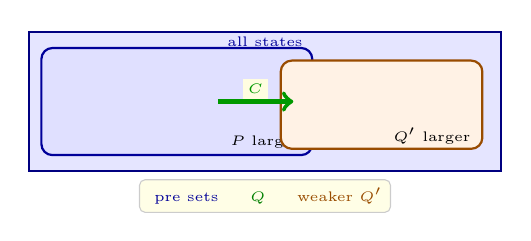
\begin{tikzpicture}[scale=0.80,font=\scriptsize]
\draw[fill=blue!10,draw=blue!50!black,thick] (0,0) rectangle (7.5,2.2);
\node[font=\tiny,blue!60!black] at (3.75,2.05) {all states};
\draw[fill=blue!20,draw=blue!60!black,thick,rounded corners=4pt] (0.4,0.35) rectangle (3.0,1.85);
\node[font=\tiny] at (1.70,1.05) {$\llbracket P'\rrbracket$};
\draw[fill=blue!12,draw=blue!60!black,thick,rounded corners=4pt] (0.2,0.25) rectangle (4.5,1.95);
\node[font=\tiny] at (3.75,0.45) {$\llbracket P\rrbracket$ larger};
\draw[fill=green!12,draw=green!50!black,thick,rounded corners=4pt] (4.2,0.45) rectangle (6.8,1.65);
\node[font=\tiny] at (5.50,1.35) {$\llbracket Q\rrbracket$};
\draw[fill=orange!10,draw=orange!60!black,thick,rounded corners=4pt] (4.0,0.35) rectangle (7.2,1.75);
\node[font=\tiny] at (6.40,0.55) {$\llbracket Q'\rrbracket$ larger};
\draw[->,ultra thick,green!60!black] (3.0,1.10) -- (4.2,1.10) node[midway,above,font=\tiny,fill=yellow!12,inner sep=2pt] {$C$};
\node[font=\tiny,align=left,fill=yellow!10,draw=gray!40,rounded corners=2pt,inner sep=3pt] at (3.75,-0.40) {\textcolor{blue!60!black}{$\blacksquare$ pre sets} \quad \textcolor{green!50!black}{$\blacksquare$ $Q$} \quad \textcolor{orange!60!black}{$\blacksquare$ weaker $Q'$}};
\end{tikzpicture}
\caption{Safe moves: shrinking the pre (stronger $P'$) and growing the post (weaker $Q'$) preserve the triple. The image of $P'$ under $C$ still lands inside $Q\subseteq Q'$.}
\label{fig:strengthen-weaken}
\end{figure}

% ============================================================
\section{Writing Good Specs and Spotting Bad Ones}
\label{sec:good-bad}
Three prototypical bad specs:

\textbf{Vacuous:} $\{ \text{false}\}\,C\,\{Q\}$—always true, tells nothing. Symptom: pre contains contradiction like $x>0\land x<0$. Fix: weaken pre until satisfiable.

\textbf{Too weak post:} $\{ \text{true}\}\,r:=\texttt{isqrt}(n)\,\{r\ge0\}$—true even for $r=999$. Fix: strengthen post until it pins down the desired answer.

\textbf{Too strong pre:} $\{ \text{sorted}(a)\land n=2^{k}\}\, \texttt{bsearch}\,\{ \text{found}\}$—excludes most arrays. Fix: weaken pre to the minimal assumption the algorithm actually needs.

\begin{example}[Binary search contract]
Good: $\{ \text{sorted}(a[0..n-1])\land 0\le n\}\; r:=\texttt{bsearch}(a,n,key)\; \{(r\ge0\Rightarrow a[r]=\!key)\land (r\!=\!-1\Rightarrow key\notin a)\}$. Every conjunct is load-bearing: sorted is needed for correctness, the two implications capture both outcomes precisely.
\end{example}

\begin{lstlisting}[language=Java, caption={JML-style contract for integer square root: the spec the code must satisfy.}, label={lst:jml-isqrt}]
/* @ requires n >= 0;
  @ ensures \result >= 0 && \result*\result <= n
  @      && n < (\result+1)*(\result+1);
  @*/
int isqrt(int n){
    int r = 0;
    while((r+1)*(r+1) <= n) r++;
    return r;
}
\end{lstlisting}

\begin{lstlisting}[language=Python, caption={Checking strength: implication as subset test on samples.}, label={lst:strength-py}]
def implies(P, Q, domain):
    """Does P => Q hold on finite domain sample?"""
    for s in domain:
        if P(s) and not Q(s):
            return False, s  # s satisfies P but not Q
    return True, None

P  = lambda s: s['x']==5
Q1 = lambda s: s['x']>0
Q2 = lambda s: s['x']>10
print(implies(P, Q1, [{'x':i} for i in range(-2,12)])) # True: 5=> >0
print(implies(P, Q2, [{'x':i} for i in range(-2,12)])) # False: counterexample x=5
\end{lstlisting}

% ============================================================
\section{Quantifiers, English, and Class Invariants}
\label{sec:quantifiers}
Specs of collections need quantifiers. ``$a$ is sorted'' abbreviates $\forall i.\,0\le i < n-1 \Rightarrow a[i]\le a[i+1]$. ``$key$ appears at $k$'' is $\exists k.\,0\le k<n\land a[k]=key$. Translating English is error-prone: ``all evens are positive'' is $\forall x.\,(even(x)\Rightarrow x>0)$, not $\forall x.\,even(x)\land x>0$ (which claims everything is even!).

A \emph{class invariant} is a condition that every public method may assume on entry and must re-establish on exit. For a sorted list object:
\[
\texttt{inv}:\ 0\le \texttt{size}\le \texttt{capacity}\ \land\ \text{sorted}(a[0..\texttt{size}-1]).
\]
The invariant is conjoined to every method's pre and post; it is the ``steady truth'' between calls. Chapter~4 will elevate this to loop invariants—the same idea, but preserved across iterations rather than method calls.

\begin{example}[Quantifier pitfalls]
Spec for ``$r$ is first occurrence of $key$'': 
\[
\{ \text{true}\}\;r:=\texttt{first}(a,key)\;\{ (r=-1\Rightarrow \forall i.\,a[i]\neq key)\ \land\ (r\ge0\Rightarrow a[r]=key\land\forall i<r.\,a[i]\neq key)\}.
\]
Dropping $\forall i<r$ gives a post that allows a later occurrence to be returned—too weak. Adding $\forall i.\,a[i]\neq key$ to the second conjunct makes it unsatisfiable when $key$ exists—too strong.
\end{example}

% ============================================================
\section{Exercises}
\label{sec:ch02-exercises}
\begin{enumerate}[label=E2.\arabic*, leftmargin=*, itemsep=0.6em]
    \item \textbf{Strength ordering.} Order by strength: $x=3$, $x\ge3$, $x>0$, $\text{true}$, $\text{false}$, $x\ge0\land x\le5$. Draw the implication lattice.
    \item \textbf{Strengthen/Weaken soundness.} Give a concrete $C$, $P$, $P'$ where $P\Rightarrow P'$ but $\{P\}\,C\,\{Q\}$ holds while $\{P'\}\,C\,\{Q\}$ fails. Explain why weakening pre is unsafe.
    \item \textbf{Sorted contract.} Write pre/post for linear search without assuming sortedness but guaranteeing the same two-case post as binary search. Compare strength of the two pres.
    \item \textbf{Spot the vacuous.} Find the vacuous triple among: (a) $\{x>0\land x<0\}\,x:=1\,\{x=1\}$, (b) $\{x\ge0\}\,x:=x+1\,\{x>0\}$, (c) $\{\text{true}\}\,\texttt{skip}\,\{\text{false}\}$. For the vacuous one, give the weakest satisfiable strengthening of pre that makes it meaningful.
    \item \textbf{JML translation.} Translate the informal ``$\texttt{divide}(a,b)$ returns $q$ with $a=bq+r$ and $0\le r<b$'' into a formal pre/post with quantifiers. What happens if you drop $b>0$ from pre?
\end{enumerate}

\section*{Chapter Notes}
Design by Contract originates with Meyer's Eiffel; JML (Leavens et~al.) brings it to Java. The lattice view of assertions is standard in abstract interpretation (Cousot). For practice, write contracts before code—specification is the hardest and most valuable part of verification.

\smallskip
\begin{remark}[Checklist for a good contract]
Ask: is $P$ satisfiable? Is $Q$ strong enough to be useful? Does $Q$ avoid claiming the unclaimable (no disjunction forgotten, no $\forall$ where $\exists$ needed)? If you cannot state $Q$ precisely, you do not yet understand what the program should do.
\end{remark}
% End of Chapter 2
